% ---------- figs/graph_sample.tex ----------
\begin{figure}[!ht]
    \centering
    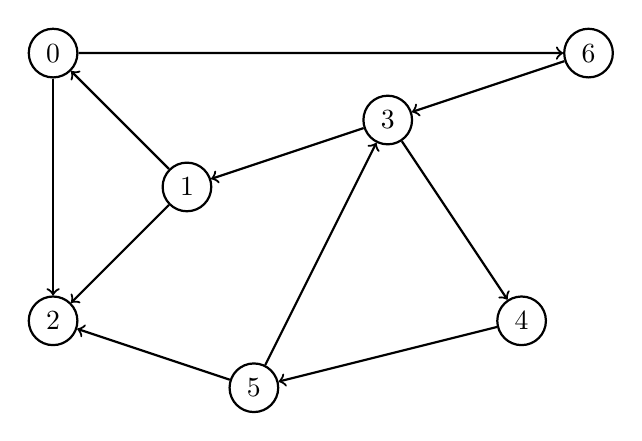
\begin{tikzpicture}[node distance={10mm}, thick, main/.style = {draw, circle}, scale=0.85] 
    
        \node [main] (0) at (-3, 3) {0};
        \node [main] (1) at (-1, 1) {1};
        \node [main] (2) at (-3, -1) {2};
        \node [main] (3) at (2, 2) {3};
        \node [main] (4) at (4, -1) {4};
        \node [main] (5) at (0, -2) {5};
        \node [main] (6) at (5, 3) {6};
    
        \draw[<-] (0) to (1);
        \draw[->] (1) to (2);
        \draw[<-] (1) to (3);
        \draw[->] (3) to (4);
        \draw[<-] (5) to (4);
        \draw[->] (5) to (3);
        \draw[<-] (3) to (6);
        \draw[<-] (6) to (0);
        \draw[->] (5) to (2);
        \draw[->] (0) to (2);
        
    \end{tikzpicture}
    \caption{A graph drawn using TikZ.}
    \label{fig:graph}
\end{figure}
